\documentclass[
Karos,
%Loesung,
%Punkte
]{pruefung}

\renewcommand{\Pruefungsfach}{\textbf{Prüfungsfach: Mathematik 2}}
\renewcommand{\Semester}{\textbf{Sommersemester 23}}
\renewcommand{\Studiengaenge}{\textbf{Studiengänge: SWB/TIB/IEP}}
\renewcommand{\Fachnummern}{\textbf{Prüfungsnummer: IT 105\;20\;03 und 105\;20\;13}}
\renewcommand{\Dauer}{\textbf{Zeit: 90 Minuten}}
\renewcommand{\Dozenten}{\textbf{Dozent: Prof. Dr. Jürgen Koch}}

\renewcommand{\Hilfsmittel}{
\textbf{Manuskript\newline
 Literatur\newline
Taschenrechner Casio FX-87DE Plus / Casio FX-87DE Plus 2nd edition}
}
\renewcommand{\Hinweise}{
\textbf{Bearbeiten Sie die Aufgaben ausschließlich auf diesen Prüfungsblättern.
\newline
Begründen Sie alle Lösungsschritte.}
}

\begin{document}
\begin{Aufgabe}[10]
Hinweis: Alle Teilaufgaben können unabhängig voneinander bearbeitet werden.

\begin{enumerate}
	\item
	Ordnen Sie den Differenzialgleichungen die Richtungsfelder zu:

\begin{tabular}{p{0.25\textwidth}p{0.25\textwidth}p{0.25\textwidth}p{0.25\textwidth}}
	(A) $y' = -y$ &
	(B) $y' = -x$ &
	(C) $y' = y^2$ &
	(D) $y' = x^2$ \\
\end{tabular}

\begin{tabular}{llll}
	\ifLoesung
	( {\textcolor{red}C} ) &
	\else
	( \quad ) &
	\fi
	\hspace*{-10mm} \raisebox{-0.8\height}{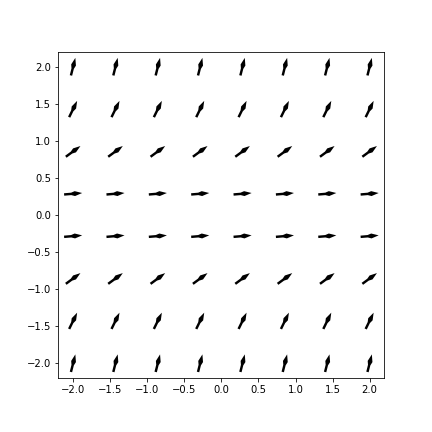
\includegraphics[width=0.4\textwidth]{../M2_IT/m2_it_ss_23_kurzaufgaben_richtungsfeld_3.png}} &
	\ifLoesung
	( {\textcolor{red}B} ) &
	\else
	( \quad ) &
	\fi
	\hspace*{-10mm} \raisebox{-0.8\height}{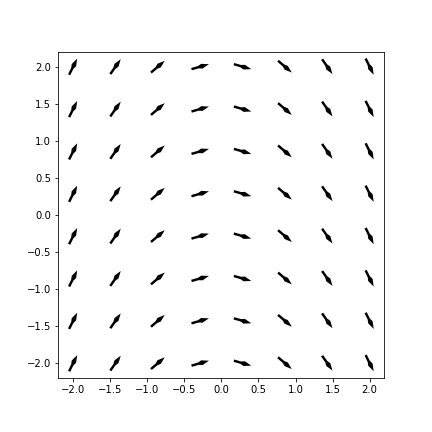
\includegraphics[width=0.4\textwidth]{../M2_IT/m2_it_ss_23_kurzaufgaben_richtungsfeld_2.png}}  \\
	\ifLoesung
	( {\textcolor{red}D} ) &
	\else
	( \quad ) &
	\fi
	\hspace*{-10mm} \raisebox{-0.8\height}{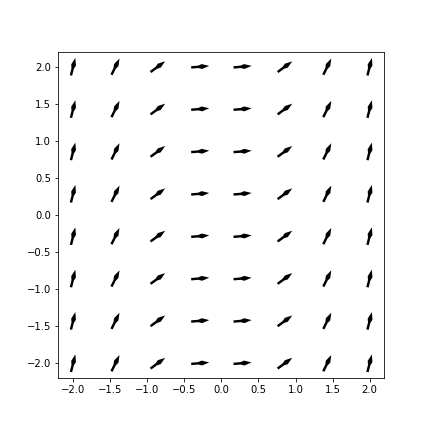
\includegraphics[width=0.4\textwidth]{../M2_IT/m2_it_ss_23_kurzaufgaben_richtungsfeld_4.png}} &
	\ifLoesung
	( {\textcolor{red}A} ) &
	\else
	( \quad ) &
	\fi
	\hspace*{-10mm} \raisebox{-0.8\height}{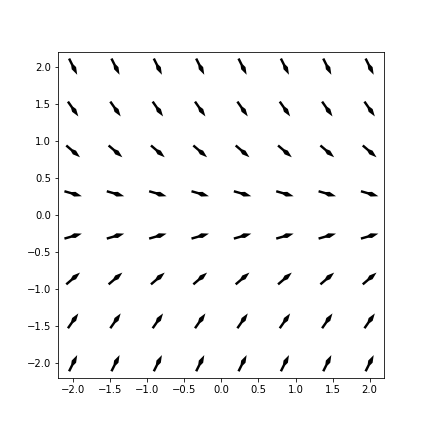
\includegraphics[width=0.4\textwidth]{../M2_IT/m2_it_ss_23_kurzaufgaben_richtungsfeld_1.png}}  \\
\end{tabular}

\ifLoesung
\mbox{}\hfill\Punkte{2 P}\\
\fi	

\pagebreak

	\item
		Welche Differenzialgleichung ist linear? Bitte kreuzen Sie den entsprechenden Eintrag an:

\ifLoesung 
\begin{tabular}{p{0.3\textwidth}p{0.2\textwidth}p{0.2\textwidth}}
	$y'' + 2 \, y' + y = \sin(x)$     & {\textcolor{red}X} linear &            $\square$ nicht linear\\
	$y'' + 2 \, y' + \sin(y) = 0$    & $\square$ linear  & {\textcolor{red}X} nicht linear\\
	$y'' + 2 \, y' + \sin(x) = 0$ &  {\textcolor{red}X} linear &            $\square$ nicht linear\\
	$y'' + 2 \, y' + \sin(x) \, y = 0$     & {\textcolor{red}X} linear &            $\square$ nicht linear\\
\end{tabular}
\hfill\Punkte{2 P}
\else
\begin{tabular}{p{0.3\textwidth}p{0.2\textwidth}p{0.2\textwidth}}
	$y'' + 2 \, y' + y = \sin(x)$     & $\square$ linear & $\square$ nicht linear\\
	$y'' + 2 \, y' + \sin(y) = 0$        & $\square$ linear & $\square$ nicht linear\\
	$y'' + 2 \, y' + \sin(x) = 0$     & $\square$ linear & $\square$ nicht linear\\
	$y'' + 2 \, y' + \sin(x) \, y = 0$ & $\square$ linear & $\square$ nicht linear\\
\end{tabular}
\fi

	\item
	Die Differenzialgleichung der Balkendurchbiegung $w(x)$ lautet:
	\[
		\frac{w''(x)}{({1 + (w'(x))^2})^{3/2}} = -\frac{M_y(x)}{E \, I_y} \, .
	\]
	Dabei bezeichnet $M_y(x)$ das Biegemoment an der Stelle $x$, $E$ das Elastizitätsmodul des Balkenmaterials und $I_y$ das axiale Flächenträgheitsmoment des Balkenquerschnitts.
	Stellen Sie die Differenzialgleichung mit Zustandsvariablen durch ein äquivalentes System von Differenzialgleichungen erster Ordnung dar.

\Loesung{}{
	Zwei Zustandsvariablen:
	\hfill\Punkte{2 P}
	\[
	z_1 = w(x), \, z_2 = w'(x) \, .
	\]
	System von Differenzialgleichungen erster Ordnung:
	\[
	\begin{array}{ccl}
		z'_1 & = & z_2 \, , \\
		z'_2 & = &  -\frac{M_y(x)}{E \, I_y} ({1 + z_2^2})^{3/2} \, .
	\end{array}
	\]
}
	
\pagebreak

	\item
		Folgende Frage wurde ChatGPT in der Version vom 12. Mai 2023 gestellt: 
		
		\begin{verbatim}
		Ein Teich enthält 1000 Liter Wasser. Täglich verdunsten 2% des Wassers im Teich und
		10 Liter Wasser werden nachgefüllt. Wieviel Wasser enthält der Teich nach 2 Tagen?
		\end{verbatim}
		
		Die Antwort lautete:
		
		\begin{verbatim}
		Zuerst berechnen wir die tägliche Verdunstungsmenge: 2% von 1000 Litern sind 20
		Liter. Da täglich 10 Liter Wasser nachgefüllt werden, verringert sich die Wasser-
		standsmenge um 10 Liter - 20 Liter = -10 Liter pro Tag. Nach 2 Tagen würde sich die
		Wassermenge im Teich um -10 Liter * 2 Tage = -20 Liter verringern. Da der Wasser-
		verlust die Nachfüllung übersteigt, enthält der Teich nach 2 Tagen kein Wasser mehr.
		\end{verbatim}
		
		Bestimmen Sie die korrekte Wassermenge im Teich nach $2$ Tagen mithilfe einer Differenzengleichung.
		
		\Loesung{5cm}{
			Differenzengleichung:
			\hfill\Punkte{2 P}
			\[
				T_{k+1} = 0.98 \, T_k + 10, \quad T_0 = 1000
			\]
			Nach einem Tag:
			\[
				T_1 = 0.98 \cdot 1000 + 10 = 990 
			\]
			Nach zwei Tagen:
			\[
				T_2 = 0.98 \cdot 990 + 10 =  980.2
			\]
			}
		
		\item
		Welchen Grenzwert $S$ hat die Reihe
		\[
			S = \sum_{k=2}^\infty \left(\frac{1}{3}\right)^k \, ?
		\]
		\Loesung{}{
			Geometrische Reihe mit $q = \frac{1}{3}$:
			\hfill\Punkte{2 P}
			\[
			\sum_{k=0}^\infty \left(\frac{1}{3}\right)^k  = \frac{1}{1 - q} = \frac{1}{1 - \frac{1}{3}} = \frac{3}{2} \, .
			\]
			Erste beiden Glieder:
			\[
				S = \sum_{k=2}^\infty \left(\frac{1}{3}\right)^k  = \sum_{k=0}^\infty \left(\frac{1}{3}\right)^k  - \left( 1 + \frac{1}{3} \right)  =   \frac{1}{6} 
			\]
		}
	\end{enumerate}

\end{Aufgabe}

\newpage

\endinput
\begin{Aufgabe}[8]% Vgl. SS 06
Gegeben ist das Anfangswertproblem 
\[
	y' = (y + 1) \, \cos(x), \quad  y(0) = 1.
\]
\begin{enumerate}
	\item
		Ist die Differenzialgleichung linear?
	\item
		Berechnen Sie die Lösung des Anfangswertproblems.   
	\item
		Ermitteln Sie einen Näherungswert $\tilde{y}_1$ für die Lösung des Anfangswertproblems an der Stelle $x=0.1$, indem Sie einen Schritt mit dem Euler-Polygonzugverfahren mit der Schrittweite $h = 0.1$ durchführen.
		Wie weit weicht der Näherungswert $\tilde{y}_1$ von der exakten Lösung ab? 
\end{enumerate}

\Loesung{}{
	\begin{enumerate}
		\item
			Linear.
			\hfill \Punkte{1 P}
		\item
			Trennung der Variablen:
			\hfill \Punkte{1 P}
			\[
				y' = (y + 1) \, \cos(x)
				\quad \Longrightarrow \quad 
				\int \frac{1}{y + 1} \, \mathrm{d}y = \int \cos(x) \, \mathrm{d}x
			\]
			Stammfunktionen:
			\hfill \Punkte{1 P}
			\[
				\ln\left(\left| y + 1 \right|\right) = \sin(x) + C_1, \quad C_1 \in \mathbb{R}
			\]
			Nach $y$ auflösen:
			\hfill \Punkte{1 P}
			\[
				\left| y + 1 \right| = \e^{ \sin(x) + C_1}
				\quad \Longrightarrow \quad 
				y + 1 = \pm \, \e^{C_1} \, \e^{ \sin(x)}
				\quad \Longrightarrow \quad
				y = C_2 \, \e^{ \sin(x)} - 1, \quad C_2 \in \mathbb{R}
			\]
		Anfangswert: 
		\hfill \Punkte{1 P}
		\[
		y(0) = C_2 - 1
		\quad \Longrightarrow \quad
		1 = C_2 - 1
		\quad \Longrightarrow \quad
		C_2 = 2
		\quad \Longrightarrow \quad
		y(x) =  2 \, \e^{ \sin(x)} - 1
		\]
		\item
		Euler-Polygonzugverfahren: 
		\hfill \Punkte{1 P}
		\[
		\tilde{y}_{n+1} = \tilde{y}_n + h \, ( \tilde{y}_n + 1) \, \cos(x_n),
		\]
		Schritt von $x_0=0$ nach $x_1=0.1$ mit Schrittweite $h=0.1$:
		\hfill \Punkte{1 P}
		\[
		\tilde{y}_1 = 1 + 0.1 \cdot (1 + 1) \, \cos(0)  = 1.2
		\]
		Abweichung:
		\hfill \Punkte{1 P}
		\[
		y(1.1) - \tilde{y}_1 = 2 \, \e^{ \sin(0.1)} - 1 - 1.2 \approx 0.009974
		\]	
	\end{enumerate}
}

\ifLoesung
\else
\newpage
\Loesung{}{}
\fi

\end{Aufgabe}

\newpage

\endinput
\begin{Aufgabe}[10]
Bestimmen Sie die allgemeine reelle Lösung der Differenzialgleichung
\[
	y'' + 4 \, y = 3 \, \cos( 2 \, x ) \, .
\]
\end{Aufgabe}

\Loesung{}{
	Charakteristische Gleichung:
	\hfill \Punkte{2 P} 
	\[
		\lambda^2 + 4 \, = 0
		\quad \Longrightarrow \quad
		\lambda_{1,2} = \pm 2 \, \mbox{i} 
	\]
	Homogene Lösung:
	\hfill \Punkte{1 P} 
	\[
		y_h(x) = C_1 \cos( 2 \, x )+ C_2 \sin( 2 \, x )
	\]
	Resonanzansatz für partikuläre Lösung:
	\hfill \Punkte{2 P} 
	\[
		y_p(x) = x \left( A \cos( 2 \, x )+ B \sin( 2 \, x ) \right)
	\]
	Erste Ableitung:
	\hfill \Punkte{1 P} 
	\[
		y'_p(x) = A \cos( 2 \, x )+ B \sin( 2 \, x ) + x \left( -2 \, A \sin( 2 \, x )+ 2 \, B \cos( 2 \, x ) \right)
	\]
	Zweite Ableitung:
	\hfill \Punkte{1 P} 
	\[
		y''_p(x) = -2 \, A \sin( 2 \, x )+ 2 \, B \cos( 2 \, x ) -2 \, A \sin( 2 \, x )+ 2 \, B \cos( 2 \, x ) 
		+ x \left( -4 \, A \cos( 2 \, x ) - 4 \, B \sin( 2 \, x ) \right)
	\]
	In Differenzialgleichung einsetzen:
	\hfill \Punkte{1 P} 
	\[
		\underbrace{-4 \, A \sin( 2 \, x )+ 4 \, B \cos( 2 \, x ) - 4\,  x \left( A \cos( 2 \, x ) + B \sin( 2 \, x ) \right)}_{\displaystyle y_p''}
		+ 4 \, 	\underbrace{x \left( A \cos( 2 \, x )+ B \sin( 2 \, x ) \right)}_{\displaystyle y_p} = 3 \, \cos( 2 \, x )
	\]
	$A$ und $B$ berechnen:
	\hfill \Punkte{1 P} 
	\[
		A = 0, \quad B = \frac{3}{4}
	\]
	Allgemeine reelle Lösung:
	\hfill \Punkte{1 P}
	\[
		y(x) = y_h(x) + y_p(x) = C_1 \cos( 2 \, x )+ C_2 \sin( 2 \, x ) +  \frac{3}{4} \, x \, \sin( 2 \, x )
	\]
}

\pagebreak

\ifLoesung
\else
\Loesung{}{}
\fi

\endinput
\begin{Aufgabe}[8] % vgl. SS 16, gleiche Matrix als DGL-System
	Gegeben ist das Differenzengleichungssystem
	\[
	\begin{array}{rcrcr}
		x_{k+1} & = & -2 \, x_k & + & 3 \, y_k,\\[1ex]
		y_{k+1} & = &	2 \, x_k & + & 3 \, y_k,\\
	\end{array}
	\quad k = 0,1,2,\ldots
	\]
	\begin{enumerate}
		\item
			Berechnen Sie die allgemeine Lösung des Differenzengleichungssystems.
		\item
			Ist das Differenzengleichungssystem asymptotisch stabil?
	\end{enumerate}
	
	\Loesung{}{
		\begin{enumerate}
			\item
			Vektor-Matrix-Form:
			\[
			\left(
			\begin{array}{l}
				x_{k+1}\\[1ex]
				y_{k+1}\\
			\end{array}
			\right)
			=
			\left(
			\begin{array}{rr}
				-2 & 3\\[1ex]
				  2 & 3\\
			\end{array}
			\right)
			\left(
			\begin{array}{l}
				x_{k}\\[1ex]
				y_{k}\\
			\end{array}
			\right)
			\hfill \Punkte{1 P} 
			\]
			Charakteristische Gleichung und Eigenwerte:
			\[
			\left|
			\begin{array}{cc}
				-2 - \lambda &                   3\\[1ex]
				                   2 & 3 - \lambda \\
			\end{array}
			\right|
			= \lambda^2 - \lambda - 12 = 0
			\quad \Longrightarrow \quad
			\lambda_1 = 4, \, \lambda_2 = -3 
			\hfill \Punkte{3 P} 
			\]		
			Eigenvektor für $\lambda_1 = 4$:
			\[
			\left(
			\begin{array}{rr}
				-6 &  3 \\[1ex]
				  2 & -1 \\
			\end{array}
			\right)
			\, \mathbf{v} = \mathbf{0}
			\quad \Longrightarrow \quad
			\mathbf{v} =
			\left(
			\begin{array}{r}
				\hphantom{-}1\\
				2\\
			\end{array}
			\right)  
			\hfill \Punkte{1 P} 
			\]  
			Eigenvektor für $\lambda_2 = -3$:
			\[
			\left(
			\begin{array}{rr}
				\hphantom{-}1 & \hphantom{-}3\\[1ex]
				2 & 6\\
			\end{array}
			\right)
			\, \mathbf{v} = \mathbf{0}
			\quad \Longrightarrow \quad
			\mathbf{v} =
			\left(
			\begin{array}{r}
				 3\\
				-1\\
			\end{array}
			\right)  
			\hfill \Punkte{1 P} 
			\]
			Allgemeine Lösung
			\[
			\left(
			\begin{array}{l}
				x_{k}\\
				y_{k}\\
			\end{array}
			\right)
			=
			C_1 \, 4^k
			\left(
			\begin{array}{r}
				\hphantom{-}1\\
									2\\
			\end{array}
			\right)   
			+ C_2 \, \left( -3 \right)^k
			\left(
			\begin{array}{r}
				3\\
				-1\\
			\end{array}
			\right)   
			\hfill \Punkte{1 P} 
			\]
			\item
			Die Beträge der Eigenwerte sind nicht kleiner als $1$.
			Somit ist das Differenzengleichungssystem nicht asymptotisch stabil.
			\hfill \Punkte{1 P} 
		\end{enumerate}
	}
	
	\ifLoesung
	\else
	\newpage
	\Loesung{}{}
	\fi
	
\end{Aufgabe} 

\newpage

\endinput
\begin{Aufgabe}[8]% vgl. WS 17/18
	Gegeben ist die Funktion $f$ mit 
	\[
		f(x)=\frac{1}{x}\ln(1+x) \, .
	\]
	\begin{enumerate}
		\item
			Geben Sie die Potenzreihe der Funktion $f$ an.
		\item
			Welchen Konvergenzradius $r$ hat die Potenzreihe aus Aufgabenteil \textbf{a)}.
		\item
			Bestimmen Sie den Grenzwert
			\[
				\lim_{x \to 0} f(x)
			\]
			mithilfe der Potenzreihe aus Aufgabenteil \textbf{a)}.
		\item
			Berechnen Sie einen Näherungswert $\tilde{I}$ für das bestimmte Integral
			\[
				I = \int_0^1 f(x) \, \mbox{d} \, x
			\]
			mithilfe der Potenzreihe aus Aufgabenteil \textbf{a)} mit allen Gliedern bis zur Ordnung $2$.
		\item
			Schätzen Sie die maximale Abweichung des Näherungswertes $\tilde{I}$ aus Aufgabenteil \textbf{d)} vom exakten Wert $I$ mithilfe des Leibniz-Kriteriums.
	\end{enumerate}
%
%
%
\Loesung{}{
	\begin{enumerate}[series=potenzreihen_loesung]
		\item
			Potenzreihe des Logarithmus:
			\hfill\Punkte{2 P}
			\[
				\ln(1 + x)	=	\sum_{k=1}^{\infty}\frac{(-1)^{k-1}}{k}x^k = x-\frac{x^2}{2}+\frac{x^3}{3}-\frac{x^4}{4} \pm \ldots
			\]
			Potenzreihe von $f$:
			\[
				f(x)
				= \frac{1}{x}  \sum_{k=1}^{\infty}\frac{(-1)^{k-1}}{k}x^k
				= \sum_{k=1}^{\infty}\frac{(-1)^{k-1}}{k}x^{k-1}
				= 1 - \frac{x}{2} + \frac{x^2}{3} - \frac{x^3}{4} \pm \ldots
			\]
		\item
			Konvergenzradius $r=1$
			\hfill\Punkte{1 P}
		\item
			Grenzwert:
			\hfill\Punkte{1 P}
			\[
				\lim_{x\to 0} f(x) = \lim_{x\to 0} \left(1 - \frac{x}{2} + \frac{x^2}{3} - \frac{x^3}{4} \pm \ldots \right) = 1
			\]
	\end{enumerate}
}

\newpage

\Loesung{}{
	\begin{enumerate}[resume=potenzreihen_loesung]
		\item
			Gliedweise Integration der Potenzreihe:
			\hfill\Punkte{2 P}
			\[
				\tilde{I}
				\approx \int_0^1 \left( 1 - \frac{x}{2} + \frac{x^2}{3} \right) \, dx 
				= \left[ x - \frac{x^2}{4} + \frac{x^3}{9} \right]_0^1
			\]
			Integrationsgrenzen:
			\[
				\tilde{I} = 1 - \frac{1}{4} + \frac{1}{9} = \frac{31}{36}
			\]
		\item
			Die Glieder der Reihe bilden eine monotone Nullfolge, deshalb kann man die Abweichung des Näherungswertes $\tilde{I}$ von der exakten Lösung $I$ mit dem Leibniz-Kriterium abschätzen.
			
			Abschätzung:
			\hfill\Punkte{2 P}
			\[
				\left| \tilde{I} - I \right|
				\leq 	\left| \int_0^1 - \frac{x^3}{4} \right| 
				= \left|  \left[  - \frac{x^4}{16} \right]_0^1 \right| = \frac{1}{16}
			\]
	\end{enumerate}
}

\end{Aufgabe}

\endinput
\begin{Aufgabe}[10]
	Gegeben ist die periodische Funktion $f$, mit
	\[
	f(t) = \e^{t/2} \mbox{ für } t \in [-\pi, \pi), \quad f(t + 2 \, \pi) = f(t) \, .
	\]
	\begin{enumerate}
		\item
			Skizzieren Sie die Funktion $f$ für $t \in [-\pi, 4 \, \pi]$.
		\item
			Bestimmen Sie eine Formel für die komplexen Fourier-Koeffizienten $c_k$ der Funktion $f$, für $k = 0,1,2,3,\ldots$
		\item
			Welchen Mittelwert $m$ hat die Funktion $f$?
		\item
			An welchen Stellen tritt bei der Funktion $f$ das Gibbsche Phänomen auf?
			Wie groß sind die Überschwinger?
	\end{enumerate}
	
	\begin{tikzpicture}[xscale=1.0,yscale=1.0]
		\draw[line width=0.25pt,step=0.5cm,color=lightgray] (-4.0,-6.0) grid(13.5cm,6.0cm);
		\draw[->,thick] (-3.5, 0.0) -- (13.0, 0.0) node[below=1mm] {$t$};
		\draw[->,thick] ( 0.0,-5.5) -- ( 0.0,5.5) node[left]  {$f$};
		\foreach \i in {-5,-4,-3,-2,-1,1,2,3,4,5} {
			\draw[thick] (0.1,\i) -- (-0.1,\i) node[left] {$\i$};
		}
		\draw[thick] (-3.14,0.1) -- (-3.14,-0.1) node[below] {$\vphantom{2}-\pi$};
		\draw[thick] (  3.14,0.1) -- (  3.14,-0.1) node[below] {$\vphantom{2}\pi$};
		\draw[thick] (  6.28,0.1) -- (  6.28,-0.1) node[below] {$2 \, \pi$};
		\draw[thick] (  9.42,0.1) -- (  9.42,-0.1) node[below] {$3 \, \pi$};
		\draw[thick] (12.56,0.1) -- ( 12.56,-0.1) node[below] {$4 \, \pi$};
		\ifLoesung
		\draw[ultra thick, smooth, domain=-3.14:3.14,color=red] plot (\x,{exp(0.5*\x)}) ;
		\draw[ultra thick, smooth, domain=3.14:9.42,color=red] plot (\x,{exp(0.5*(\x-6.28))}) ;
		\draw[ultra thick, smooth, domain=9.42:12.56,color=red] plot (\x,{exp(0.5*(\x-12.56))}) ;
		\fi
	\end{tikzpicture}
	
	\Loesung{}{
		\begin{enumerate}[series=fourierreihen_loesung]
			\item
			Skizze:
			\hfill\Punkte{2 P}
		\end{enumerate}
	}
	
	\newpage
	
	\Loesung{}{
		\begin{enumerate}[resume=fourierreihen_loesung]
			\item
			Formel:
			\hfill\Punkte{1 P}
			\[
			c_k
			= \frac{1}{T} \int_{-T/2}^{T/2} f(t) \, \e^{- \mathrm{i} \, k \, \omega \, t}  \mathrm{d} \, t
			= \frac{1}{2 \, \pi} \int_{-\pi}^{\pi} \e^{t/2}  \e^{- \mathrm{i} \, k \, t}  \mathrm{d} \, t \, .
			\]
			Stammfunktion:
			\hfill\Punkte{2 P}
			\[
			c_k
			= \frac{1}{2 \, \pi} \int_{-\pi}^{\pi} \e^{t/2 - \mathrm{i} \, k \, t}  \mathrm{d} \, t
			= \frac{1}{2 \, \pi} \int_{-\pi}^{\pi} \e^{\left(1/2 - \mathrm{i} \, k \right) t}  \mathrm{d} \, t
			= \frac{1}{2 \, \pi} \left[ \frac{ \e^{\left(1/2 - \mathrm{i} \, k \right) t} }{1/2 - \mathrm{i} \, k } \right]_{- \, \pi}^\pi \, .
			\]
			Grenzen einsetzen und vereinfachen:
			\hfill\Punkte{2 P}
			\[
			c_k
			= \frac{ \e^{\left(1/2 - \mathrm{i} \, k \right) \pi} -  \e^{\left(1/2 - \mathrm{i} \, k \right) (- \pi)}}{2 \, \pi \left(1/2 - \mathrm{i} \, k \right)}
			= \frac{ \e^{\pi / 2- \mathrm{i} \, k \, \pi} - \e^{- \pi / 2 + \mathrm{i} \, k \, \pi}}{\pi - \mathrm{i} \, k \, 2 \, \pi}
			= \frac{ (-1)^k(\e^{\pi / 2}  - \e^{-\pi / 2} )}{\pi - \mathrm{i} \, k \, 2 \, \pi} \, .
			\]
			\item
			Mittelwert
			\hfill\Punkte{1 P}
			\[
			m
			= c_0
			=  \frac{\e^{\pi / 2}  - \e^{-\pi / 2}}{\pi} \approx 1.465 \, .
			\]
			\item
			Gibbsche Phänomen:
			\hfill\Punkte{1 P}
			\[
			t_k = \pi + k \cdot 2 \, \pi, \quad k = 0,1,2,3, \ldots \, .
			\]
			Überschwinger:
			\hfill\Punkte{1 P}
			\[
			\pm 0.09 \cdot (\e^{\pi / 2} - \e^{-\pi / 2}) \approx \pm 0. 41 \, .
			\]
		\end{enumerate}
	}
	
\end{Aufgabe}

\newpage

\endinput
\end{document}
